% Template for ICIP-2019 paper; to be used with:
%          spconf.sty  - ICASSP/ICIP LaTeX style file, and
%          IEEEbib.bst - IEEE bibliography style file.
% --------------------------------------------------------------------------

\documentclass{article}

% Two Column Compatible, Variable Width Algorithm Environments
% Written by Daniel Herber
% Based on modifications to the stack exchange answer at
% http://tex.stackexchange.com/questions/23296/setting-caption-rule-width-in-algorithm2e-algs/39574

% inputs
% 1 : float specifiers (htbp!)
% 2 : algorithm width (length)
% 3 : indent width (length)

% column environment
% \begin{vAlgorithm}[float specifiers]{algorithm width}{indent width}
% \end{vAlgorithm}

% page environment
% \begin{vAlgorithm*}[float specifiers]{algorithm width}{indent width}
% \end{vAlgorithm*}

% required packages
\usepackage[linesnumbered]{algorithm2e}

\SetKw{Continue}{continue}
\SetKw{Break}{break}
\SetKw{From}{from}
\SetKw{Import}{import}
\SetKw{As}{as}
\SetKw{Global}{global}
\SetKw{AndL}{and}
\SetKw{OrL}{or}

\SetKwProg{Def}{function}{}{end\ function}

\usepackage{etoolbox}
\usepackage{xstring}
\usepackage{calc}

% define lengths
\newlength{\xalgowidth}
\newlength{\xalgoremainder}
\newlength{\xindentwidth}

% define vAlgorithm* environment
\newenvironment{vAlgorithm*}[3][]{% before
  \setlength{\xalgowidth}{#2} % set algorithm width from second input
  \setlength{\xindentwidth}{#3} % set indent width from third input
  \setlength{\xalgoremainder}{\textwidth-\xalgowidth} % calculate indent to center the float
  \SetCustomAlgoRuledWidth{\xalgowidth} % set the rule width
  \IncMargin{\xindentwidth}
  \begin{algorithm*}[#1]
}% end before
{% after
  \end{algorithm*}
  \DecMargin{\xindentwidth}
}% end after

% define vAlgorithm environment
\newenvironment{vAlgorithm}[3][]{% before
  \setlength{\xalgowidth}{#2} % set algorithm width from second input
  \setlength{\xindentwidth}{#3} % set indent width from third input
  \setlength{\xalgoremainder}{\columnwidth-\xalgowidth} % calculate indent to center the float
  %\SetCustomAlgoRuledWidth{\xalgowidth} % set the rule width
  \SetCustomAlgoRuledWidth{\columnwidth} % set the rule width
  \IncMargin{\xindentwidth}
  \begin{algorithm}[#1] % column
}% end before
{% after
  \end{algorithm} % column
  \DecMargin{\xindentwidth}
}% end after

% redefine algorithm commands
\makeatletter
\patchcmd{\@algocf@start}{%
\begin{lrbox}{\algocf@algobox}%
}{%
\rule{0.5\xalgoremainder}{\z@}% indent
\begin{lrbox}{\algocf@algobox}%
\begin{minipage}{\xalgowidth}%
}{}{}
\patchcmd{\@algocf@finish}{%
\end{lrbox}%
}{%
\end{minipage}%
\end{lrbox}%
}{}{}
\makeatother


\usepackage{spconf,amsmath,graphicx}
\usepackage{multicol, blindtext} % add here
\usepackage{booktabs}
\usepackage{xcolor}
%\usepackage[linesnumbered,boxed]{algorithm2e}
\newcommand\mycommfont[1]{\footnotesize\ttfamily\textcolor{blue}{#1}}
\SetCommentSty{mycommfont}

% Example definitions.
% --------------------
\def\x{{\mathbf x}}
\def\L{{\cal L}}

% Title.
% ------
\title{SYMBOLIC PROGRAM SLICING ON SMART CONTRACTS}
%
% Single address.
% ---------------

\name{Zi Xuan Chen, Fang Yu}
\address{National Chengchi University \\
Department of Computer Science, Management Information Systems \\
104703010@nccu.edu.tw, yuf@nccu.edu.tw}

%
% For example:
% ------------
%\address{School\\
%	Department\\
%	Address}
%
% Two addresses (uncomment and modify for two-address case).
% ----------------------------------------------------------
%\twoauthors
%  {Zi Xuan Chen
%    %\sthanks{The fourth author performed the work while at ...}
%  }
%	{National Chengchi University, \\ Department of Computer Science \\
%	s10410@nccu.edu.tw}
%  {Fang Yu
%    %\sthanks{Thanks to XYZ agency for funding.}
%  }
%	{National Chengchi University, \\ Department of Management Information Systems, \\
%	yuf@nccu.edu.tw}


\begin{document}
%\ninept
%

\maketitle

%

\begin{abstract}

  %we propose a method to do program slicing. with slicing, we can analyse properties more efficiently.

  We propose a method to do program slicing on stack-based programming language. With slicing, we can analyse properties more efficiently. We take the EVM bytecode\cite{wood2014ethereum} as the example language, which is used to write smart contract\cite{szabo2003advances} on Ethereum\cite{wood2014ethereum}.

\end{abstract}

\begin{keywords}
  BlockChain, Ethereum, Slicing, Verification
\end{keywords}


\section{Introduction}
\label{sec:introduction}

There are many interest properties about Ethereum. Ethereum can be viewed as a transaction-based state machine. We can transit the transation state by sending transation or execute smart contract. On Ethereum, all transaction executed on Ethereum Virtual Machine (EVM), which is a simple stack-based architecture, limits stack item size to 1024. The word size of the machine (and thus size of stackitems) is 256-bit. Executions will be failed if stackoverflow occured while executing the smart contract. Besides stack, \textbf{\textit{gas}} is another interesting property on Ethereum. To limit the cost of the transaction execution, EVM takes the handling fee named \textbf{\textit{gas}} from transaction sender.

To analyze the properties more precisely, we slice the smart contract by construcing dependency graph (DG). With the dependencies, we can slice a smaller program from some interested point. Then we can the the sliced program for other analysis purpose.

\section{Related Work}
\label{sec:relatedwork}

TBC.

\section{Method}
\label{sec:method}

To compute the dependencies between instructions, we need construct the control flow graph (CFG) first. Unlike register-based machine's instruction, which's operand are called as register explicitly, for the stack-based machine, the operand that instructions depended are stored on the stack implicitly. Thus, a CFG for stack simulation is needed.

\RestyleAlgo{algoruled} % ruled algorithm
\begin{vAlgorithm}[]{0.50\textwidth}{1em}
  %{algorithm width}{indent width}
  \SetNoFillComment
  \caption{buildCFGandStackDependency}
  \KwIn{$Opcode$}
  \KwOut{$CFG, StackDG$}
  %\tcc{split blocks with $JUMP$, $JUMPI$, \\ $STOP$, $SELFDESTRUCT$, $RETURN$, \\ $REVERT$, $INVALID$, $SUICIDE$ \\ $JUMPDEST$ ... etc}
  \Def{buildCFGandStackDependency(opcode)}{
    dg, cfg = DG(opcode), CFG(opcode)\;
    cfg.buildBasicBlocks()\;
    cfg.buildSimpleEdges()\;
    cfg.buildFunctions(cfg.basicBlocks.first)\;
    \For{func $\in$ cfg.functions}{
      valueSetAnalysis(cfg, dg, func)\;
    }
    \Return cfg, dg\;
  }
  \tcc{state constructor}
  \Def{State()}{
    this.visit = dict(dflt=0)\;
    this.stacksIn = dict(dflt=None)\;
    this.stacksOut = dict(dflt=None)\;
    this.discoveredTargets = dict(dflt=$\O$)\;
    this.lastDiscoveredTargets = dict(dflt=$\O$)\;
  }
  \tcc{value set analysis}
  \Def{valueSetAnalysis(cfg, dg, func)}{
    stat = State()\;
    toExplore = \{ func.entry \}\;
    \Do{toExplore}{
      outBlocks = \{ toExplore.pop() \}\;
      \Do{outBlocks}{
        outBlocks = outBlocks $\cup$ \\ \quad \quad transFuncBlock(cfg, dg, func, \\ \quad \quad \quad \quad \quad \quad outBlocks.pop(), stat)\;
      }
      \For{src, dsts $\in$ stat.lastDiscoveredTargets}{
        cfg.addEdges(src, dsts)\;
        toExplore = toExplore $\cup$ dsts\;
      }
      stat.visit = dict(dflt=0)\;
      stat.lastDiscoveredTargets = dict(dflt=$\O$)\;
    }
    %cfg.computeReachability(func.entry, func.id)\;
  }

\end{vAlgorithm}

The first step to construct CFG is spliting basic blocks. We split basic blocks by \textbf{\textit{JUMPDEST}} and \textbf{\textit{end instructions}}. \textbf{\textit{JUMPDEST}} is normally considered as the beginning of blocks becuase other blocks can target \textbf{\textit{JUMPDEST}} to connect the edges. The \textbf{\textit{end instructions}} include \textbf{\textit{STOP}}, \textbf{\textit{SELFDESTRUCT}}, \textbf{\textit{RETURN}}, \textbf{\textit{REVERT}}, \textbf{\textit{INVALID}}, \textbf{\textit{SUICIDE}}, \textbf{\textit{JUMP}}, \textbf{\textit{JUMPI}}.

The second step is building the edges between basic blocks. Some edges can be computed by simply succeeding the pc of the \textbf{\textit{JUMPI}} and other instructions $\notin$ \textbf{\textit{end instructions}}, followed by \textbf{\textit{JUMPDEST}}. Because the property of the stack-based machine, all the jump destinations are pushed to stack implicitly. For this problem, we use value set analysis (VSA) to find all the possible destination values.

Most of smart contracts are written in Solidity, whcih is an object-oriented (or contract-oriented), high-level language for implementing smart contracts. The contract in Solidity is like an object. Users can call the public functions in the contract, which we can treat as member functions in a object. From lower-level --- EVM bytecode, the Solidity compiler will compile a dispatcher to dispatch public functions in the contract. The dispatcher can recognize the function hashes in transactions that users sent via Application Binary Interface (ABI). We compute the function boundaries and apply the VSA on each function to construct complete contract flow graph and instruction dependencies.



In the VSA, we traverse the basic blocks in CFG and continue finding new target address of next block by simulate the execution of instructions with a abstract stack. Abstract stack abstracts all the possible statck state. The nth-item in abstract stack represent a set of all possible value of nth-item in all possible stack state. So it is a over-approximation to compute the jump destinations. For each block, we record the states of the abstract stack before and after executing the instructions in the block. With the states, we can check the convergence of the analysis. If we revisit a block, and it's post-execution state is same as last time, we consider it achieve the convergence. We assume no new value would be found. Note that only the \textbf{\textit{PUSH}}, \textbf{\textit{SWAP}}, \textbf{\textit{DUP}}, \textbf{\textit{AND}} are implemented here, for other instructions, we only do the push, pop on the stack based on the operation times it defined. It's because other instructions implementation will not affect the target address computation.


The instructions dependencies are also constructed while doing VSA. To build the dependencies, we need keeping track of the data flow of operands. All the operands are pushed into and poped from the stack. Instead of marking the operands with the instructions which pushed it, we push the instructions to the stack directly, and edges are added when the instructions are popped. Note that we don't use abstract stack here.Instead, we use a set of stack to keep all the states of possible stacks to maintain the accuracy of each operand list. If we use abstract stack here, more combination of operand list will be generated. It will lead more ambiguous result for address evaluation while building memory dependency.

\RestyleAlgo{algoruled} % ruled algorithm
\begin{vAlgorithm}[]{0.5\textwidth}{1em}
  \SetNoFillComment
  %{algorithm width}{indent width}
  \caption{ValueSetAnalysisUtility}

  \tcc{trasfer function blocks}
  \Def{transFuncBlock(cfg, dg, func, block, stat)}{
    \uIf{(func.id = DISPATCHER\_ID \\ \quad \quad \quad \quad \AndL block.reacheable) \\ \quad \OrL stat.visit[block] $>\ visitLimit$}{ \Return\; }

    stat.visit[block] += 1\;

    \tcc{save pre-stack to check convergence}
    prevStack, \_ = stat.stacksOut[block]

    oprdStack, instStack = abstStack(), listStack()\;

    inBlocks = [b $\in$ block.inBlocks \\ \quad \quad \quad \quad \quad \quad $|$ stat.stacksOut[b] $\neq$ None]

    \For{father $\in$ inBlocks}{
      ostk, istk = stat.stacksOut[father]\;
      oprdStack = oprdStack.merge(ostk)\;
      instStack = oprdStack.merge(istk)\;
    }
    \tcc{ explore the block }
    exploreBlock(dg, block, \\ \quad \quad \quad oprdStack, instStack, stat)\;
    \tcc{ add branch according the result }
    \uIf{block.end $\in$ \{JUMP, JUMPI\}}{
      oprdStack, \_ = stat.stacksIn[end]\;
      \For{ dst $\in$ oprdStack.top().vals()}{
        \uIf{isJumpDest(dst)}{
          addBranch(src, dst, stat)\;
        }
      }
    }
    oprdStack, \_ = stat.stacksOut[end]\;
    \uIf{prevStack $\neq$ oprdStack}{
      \tcc{ not converged }
      \Return block.outBlocksByFunc(func.id)\;
    }
    \Return $\O$;
  }

  \tcc{explore basic block}
  \Def{exploreBlock(dg, block, oprdStack, instStack, stat)}{
    \For{inst $\in$ block.instructions}{
      stat.stacksIn[inst] = (oprdStack, instStack)\;
      stat.stacksOut[inst] = transferFuncInst( \\ \quad \quad \ \ dg, inst, oprdStack, instStack, stat)\;
    }
  }
  \tcc{add branch to value set analysis}
  \Def{addBranch(src, dst, stat)}{
    \uIf{dst $\notin$ stat.discoveredTargets[src]}{
      \uIf{src $\notin$ stat.lastDiscoveredTargets}{
        stat.lastDiscoveredTargets[src] = $\O$\;
      }
      stat.lastDiscoveredTargets[src].add(dst)\;
      stat.discoveredTargets[src].add(dst)\;
    }
  }

\end{vAlgorithm}

After building the instruction dependency with stacks by value set analysis. we start to build the dependency between instruction by address of memory and storage.

Memory and storage are other two main data read/write mechanisms on Ethereum except stack, where the memory is volatile, the storage is non-volatile. By the way, according the figure below, we can find that the EVM does not follow the standard von Neu-mann architecture. Rather than storing program code in generally-accessible memory or storage, it is stored separately in a virtual ROM interactable only through a specialised instruction.\cite{wood2014ethereum}


\RestyleAlgo{algoruled} % ruled algorithm
\begin{vAlgorithm}[t!]{0.5\textwidth}{1em}
  \SetNoFillComment
  %{algorithm width}{indent width}
  \caption{ValueSetAnalysisUtility}
  \tcc{ transfer instruction }
  \Def{transferFuncInst(dg, inst, \\ \quad \quad \quad \quad \quad \quad oprdStack, instStack, stat)}{
    oprdStack = oprdStack.copy()\;
    instStack = instStack.copy()\;
    \uIf{ inst $\in$ PUSHn[n=1..32] }{
     oprdStack.push(inst.operand)\;
     instStack.push(inst)\;
    }
    \uElseIf{ inst $\in$ SWAPn[n=1..16]}{
      oprdStack.swap(n)\;
      instStack.swap(n)\;
    }
    \uElseIf{ inst $\in$ DUPn[n=1..16]}{
      oprdStack.dup(n)\;
      instStack.dup(n)\;
    }
    \uElseIf{ inst = AND }{
      v1, v2 = oprdStack.pop(), oprdStack.pop()\;
      oprdStack.push(absAnd(v1, v2))\;
      v1s, v2s = instStack.pop(), instStack.pop()\;
      \For{ v1, v2 $\in$ zip(v1s, v2s)}{
        dg.addEdges(inst, [v1, v2])\;
      }
      instStack.push(inst)\;
    }
    \uElse{
      \RepTimes{inst.popTimes}{
        oprdStack.pop()\;
      }
      \For{args $\in$ [instStack.pop() \\ \quad \quad \ $|$ n $\in$ range(inst.popTimes)]$^T$}{
        dg.addEdges(inst, args)\;
      }
      \RepTimes{inst.pushTimes}{
        oprdStack.push(None)\;
        instStack.push(inst)\;
      }
    }
    \Return oprdStack, instStack\;
  }
\end{vAlgorithm}

\begin{figure}[ht!]
\centering
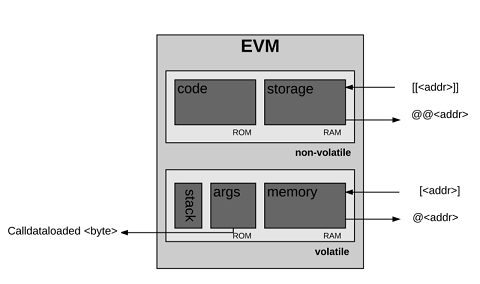
\includegraphics[width=80mm]{EVM.png}
\caption{EVM architecture\label{overflow}}
\end{figure}

There is an indexer recording current memory used, it indicates the maximum index of current memory used. The total fee for memory-usage payable is proportional to smallest multiple of 32 bytes  that  are  required  such  that  all  memory  indices (whether for read or write) are included in the range\cite{wood2014ethereum}.

Storage fees have a slightly nuanced behaviour—to in-centivise minimisation of the use of storage (which corre-sponds directly to a larger state database on all nodes),the execution fee for an operation that clears an entry in the storage is not only waived, a qualified refund is given;in fact, this refund is effectively paid up-front since the initial usage of a storage location costs substantially more than normal usage\cite{wood2014ethereum}.

The main idea to construct address dependency is traversing the CFG from write instructions with a adress, and build the dependencies with the instructions which read the address, until meet the next instructions whcih rewrite the address. With the DG we constructed, we can evaluate some address values and the stored values from known constants by the dependencies. There are some instructions about the read/write operation on memory and storage. For the storage, the write instructions is \textbf{\textit{SSTORE}}, the load instruction is \textbf{\textit{SLOAD}}. For the memory, the write instruction is \textbf{\textit{MSTORE}}, the read instruction include \textbf{\textit{MLOAD}}, \textbf{\textit{SHA3}}, \textbf{\textit{CREATE}}, \textbf{\textit{CALL}}, \textbf{\textit{RETURN}}.

For write instructions, there are three parts we concerned: the address it stored, the range of memory (offset) it covered and the value it wrote. For each part, if we could eval it as constants from other constants (normally come from the terminal of DG --- \textbf{\textit{PUSH}} instruction), we save the values as a concrete value set for the part. if not, all the instruction that it needed to do evaluation, would be saved as a dependant instruction set, once all the instruction in the set are evaluated, the part could be evaluated again to get the concrete values. Same as the write instructions, the read instructions also have these part. But for the values it load, are depended on the write instructions' value which have the same address as it, that's just the dependency we want to construct.

To build the address dependency, we new an environment which contains the three parts for the read/write instructions. we eval the storage and memory separately, but in some situations, the \textbf{\textit{SSTORE}} will dependent on some \textbf{\textit{MLOAD}} instructions, so we put both part into same evaluation loop.

\RestyleAlgo{algoruled} % ruled algorithm
\begin{vAlgorithm}[ht!]{0.56\textwidth}{1em}
  \SetNoFillComment
  %{algorithm width}{indent width}
  \caption{AnalysisEnvironment}

  \tcc{Environment constructor}

  \Def{Environment(stackDg)}{

    rInsts = stackDg.rInsts \;
    wInsts = stackDg.wInsts \;
    addrs = [ i, eval(i.addrs) $|$ i $\in$ rInsts $\cup$ wInsts ] \;
    offsets = [ i, eval(i.offsets) $|$ i $\in$ rInsts $\cup$ wInsts ] \;
    vals = [ i, eval(i.vals) $|$ i $\in$ wInsts ] \;

    \tcc{eval instructions' parameters (addr)}
    this.conAddrs = \{ i: con $|$ (i, (con, \_)) $\in$ addrs \}\;
    this.addrDepInsts = \{ i: dep $|$ (i, (\_ , dep)) $\in$ addrs \}\;

    \tcc{eval instructions' parameters (offset)}

    this.conOffsets = \{ i: con $|$ (i, (con, \_)) $\in$ offsets \}\;
    this.offsetDepInsts = \{ i: dep $|$ (i, (\_ , dep)) $\in$ offsets \}\;

    \tcc{eval instructions' parameters (val)}
    this.conVals = \{ i: con $|$ (i, (con, \_)) $\in$ vals \}\;
    this.valDepInsts = \{ i: dep $|$ (i, (\_ , dep)) $\in$ vals \}\;

    \tcc{write insts that can't be re-evaled}
    this.evaled = \{i $\in$ addrDepInsts $|$ addrDepInsts[i] = $\O$\} \\
    \quad $\cap$ \{i $\in$ offsetDepInsts $|$ offsetDepInsts[i] = $\O$\} \\
    \quad $\cap$ \{i $\in$ valDepInsts $|$ valDepInsts[i] = $\O$\}
  }

  \tcc{Return All dependant program counters}

  \Def{depInsts(env, inst)}{
    \Return env.addrDepInsts[inst] \\ \quad \quad \quad $\cup$ env.offsetDepInsts[inst] \\ \quad \quad \quad $\cup$ env.valDepInsts[inst]
  }

  \tcc{check insts if have same addr parameters }

  \Def{addrOverlap(env, instA, instB)}{
    rangeA = product(env.conAddrs[instA], \\ \quad \quad \quad \quad \quad \quad \quad \ \ env.conOffsets[instA])\;
    rangeB = product(env.conAddrs[instB], \\ \quad \quad \quad \quad \quad \quad \quad \ \ env.conOffsets[instB])\;
    \For{(Aa, Ao), (Ba, Bo) $\in$ product(rangeA, rangeB)}{
      \uIf{\{Aa..Aa + Ao\} $\cap$ \{Ba..Ba + Bo\} $\neq$ $\O$}{
        \Return True\;
      }
    }
    \Return False\;
  }

\end{vAlgorithm}

In the environment, there is a set name \textit{evaled}, which contains the instructions which's all possible values we have already evaled and stored in the concrete set, and their dependent instruction set are empty. For every evaluation round of storage and memory we check the \textit{evaled} set to determine if it achieved the convergence. If there are no new instruction added to \textit{evaled}, the evaluation will terminate.

To build the address dependency, we need to evaluate the address of the instruction first. After having some concrete addresses of write instructions, we start the CFG traversing with deep first search (DFS) from the addresses.


\RestyleAlgo{algoruled} % ruled algorithm
\begin{vAlgorithm}[]{0.52\textwidth}{1em}
  %{algorithm width}{indent width}
  \SetNoFillComment
  \caption{buildAddressDependency}
  \KwIn{$CFG$, $StackDG$}
  \KwOut{$AddressDG$}

  \Import AnalysisEnvironment \As env

  \Def{buildAddressDependency(cfg,\\ \quad \quad \quad \quad \quad \quad stackDg, opcode)}{
    \tcc{declare and alias variables}
    addrDg = DG(opcode)\;
    visit, alter = $\O$, $\O$ \;
    swrites = \{ inst $\in$ stackDg $|$ inst = SSTORE \} \;
    sreads = \{ inst $\in$ stackDg $|$ inst = SLOAD \} \;
    mwrites = \{ insts $\in$ stackDg $|$ inst = MSTORE \}\;
    mreads = \{ inst $\in$ stackDg $|$ inst $\in$ \{ MLOAD, \\ \quad \quad \quad \quad \quad SHA3, CREATE, CALL, RETURN\}\}\;

    \tcc{new a environment}
    env = Environment(stackDg)\;
    \tcc{evaluate until it converge }
    \While{True}{
      evaled = env.evaled.copy()\;
      buildDependency(addrDg, \\ \quad \quad \quad \quad swrites, sreads, visit)\;
      buildDependency(addrDg, \\ \quad \quad \quad \quad mwrites, mreads, visit)\;
      \uIf{exist write inst can be re-evaled}{
        \For{inst $\in$ re-evaled}{
          update $Environment$ $variables$ in env \\ \quad  with eval($instruction$ $parameters$)
        }
      }
      \uIf{env.evaled $\setminus$ evaled = $\O$}{
        \Break\;
      }
    }
    \Return addrDg\;
  }

  \tcc{ build dependency with write instructions}
  \Def{buildDependency(addrDg, writes, reads, visit)}{

    concrete = \{inst $\in$ (writes $\setminus$ visit) \\ \quad \quad \quad \quad \quad \quad \ \ $|$ \ \ $depInsts(env, inst)$ = $\O$\}\;
    \While{concrete $\neq$ $\O$}{

      \For{inst $\in$ concrete}{
        block = CFG.blockOf(inst)\;
        dfsCFG(addrDg, inst, block, \\ \quad \quad \quad \quad \quad writes, reads, $\O$)\;
      }
      visit.update(concrete)\;
      \For{inst $\in$ (writes $\setminus$ visit)}{
        \uIf{(depInsts(env, inst) $\setminus$ env.evaled) = $\O$}{
          update $Environment$ $variables$ in env \\ \quad with eval($instruction$ $parameters$)
        }
      }

      concrete = \{inst $\in$ (writes $\setminus$ visit) \\ \quad \quad \quad \quad \quad \quad \ \ \ $|$ \ \ $depInsts(env, ins)$ = $\O$\}\;
    }
  }
\end{vAlgorithm}

\RestyleAlgo{algoruled} % ruled algorithm
\begin{vAlgorithm}[ht!]{0.57\textwidth}{1em}
  %{algorithm width}{indent width}
  \SetNoFillComment
  \caption{dfsCFG}

  \Import AnalysisEnvironment \As env

  \tcc{do CFG dfs for building dependency}
  \Def{dfsCFG(addrDg, wInst, block, writes, reads, visit)}{
    visit.add(block)\;
    rwInsts = block.insts $\cap$ (writes $\cup$ reads)\;
    \uIf{wInst $\in$ block}{
      rwInsts = rwInsts $\setminus$ \\ \quad \quad \{ inst $\in$ block.insts $|$ inst.pc $<$ wInst.pc\}\;
    }
    \For{inst $\in$ rwInsts}{
      \tcc{if "exist the probability" to re-write the same address then return, "probability" means the "or" part}
      \uIf{inst.name = wInst.name
        \\ \quad \AndL (addrOverlap(env, wInst, inst) \\ \quad \quad \quad \OrL env.addrDepInsts[inst] $\neq$ $\O$)}{
        visit.remove(block)\;
        \Return;
      }
      \uIf{inst $\in$ reads}{
        deps = env.addrDepInsts[inst] $\cup$ \\ \quad \quad \quad \quad \ env.offsetDepInsts[inst]\;
        \uIf{deps $\neq$ $\O$ \AndL \\
          \quad  deps $\setminus$ env.evaled = $\O$}{
          update $Environment$ $variables$ in env \\ \quad \quad with eval($instruction$ $parameters$)
        }

        \uIf{addrOverlap(env, wInst, inst)}{
          env.evaled.add(inst)\;
          addrDg.addEdge(wInst, inst)\;
          env.conVals[inst].update(\\
          \quad \quad \quad \quad \quad \quad \ \ env.conVals[wInst]);
        }
      }
    }
    \For{nextBlock $\in$ block.outBlock}{
      dfsCFG(wInst, nextBlock, writes, reads, visit)\;
    }
    visit.remove(block)\;
  }

\end{vAlgorithm}

\RestyleAlgo{algoruled} % ruled algorithm
\begin{vAlgorithm}[ht!]{0.55\textwidth}{1em}
  %{algorithm width}{indent width}
  \SetNoFillComment
  \caption{eval}
  \KwIn{$instruction$, $visit$}
  \KwOut{$concrete$ $values$, $dependant$ $PCs$}

  \Def{eval(inst, visit)}{
    \uIf{inst $\in$ visit}{
      \Return $\O$, \{inst\}\;
    }
    visit.add(inst)\;
    concrete, dependant = $\O$, $\O$\;
    \uIf{inst.name.startswith('PUSH')}{
      \Return \{int(op.operand)\}, $\O$;
    }
    cons, deps = \{map(eval(\_ , visit), argList) \\ \quad \quad \quad \quad \quad \quad \quad \quad $|$ argList $\in$ inst.argLists\}$^T$\;
    \For{argList $\in$ cons}{
      val = None\;
      \uIf{None $\in$ argList}{\Continue\;}
      \uElseIf{inst.name = 'ADD'}{
        val = \Let x, y = argList \In x + y\;
      }
      \uElseIf{inst.name = 'SUB'}{
        val = \Let x, y = argList \In x - y\;
      }
      \uElseIf{inst.name = 'MUL'}{
        val = \Let x, y = argList \In x * y\;
      }
      \uElseIf{inst.name = 'DIV'}{
        val = \Let x, y = argList \In x / y\;
      }
      \uElseIf{inst.name = 'EXP'}{
        val = \Let x, y = argList \In $x^{y}$\;
      }
      \uElseIf{inst.name = 'ISZERO'}{
        \[
        val = \Let [x] = argList \ \In
          \begin{cases}
            0,& \text{if } x = 0\\
            1,              & \text{otherwise}
          \end{cases}\;
        \]
      }
      \uElseIf{inst.name = 'NOT'}{
        val = \Let [x] = argList \In (1 $<<$ 256) - 1 - x\;
      }
      \uElseIf{inst.name = 'AND'}{
        val = \Let x, y = argList \In $x \ \& \ y$\;
      }
      \uElseIf{inst.name = 'OR'}{
        val = \Let x, y = argList \In $x \ | \ y$\;
      }
      \uElseIf{inst.name = 'EQ'}{
        val = \Let x, y = argList \In $x \ = \ y$\;
      }
      \uElseIf{inst.name $\in$ \{'MLOAD', 'SLOAD', 'SHA3'\}}{
        concrete.update(env.conVals[inst])\;
      }
      \uElse{
        \tcc{SHA3 not impl yet}
        throw Exception("not handle the inst yet")\;
      }
      \uIf{val $\neq$ None}{ concrete.add(val)\; }
      dependant.update(concat(deps))\;
    }
    visit.remove(inst)\;
    \Return concrete, dependant\;
  }

\end{vAlgorithm}

\section{experiment}
\label{sec:experiment}

\section{Conclusion}
\label{sec:conclusion}

% To start a new column (but not a new page) and help balance the last-page
% column length use \vfill\pagebreak.
% -------------------------------------------------------------------------
%\vfill
%\pagebreak

% References should be produced using the bibtex program from suitable
% BiBTeX files (here: strings, refs, manuals). The IEEEbib.bst bibliography
% style file from IEEE produces unsorted bibliography list.
% -------------------------------------------------------------------------
\bibliographystyle{IEEEbib}
\bibliography{strings,refs}

\end{document}
